\documentclass[tikz,border=8pt]{standalone}
\usepackage{amsmath}
\usepackage{pgfplots}
\pgfplotsset{compat=1.18}
\usetikzlibrary{calc,arrows.meta,positioning}
\newcommand{\rad}{2}
\begin{document}
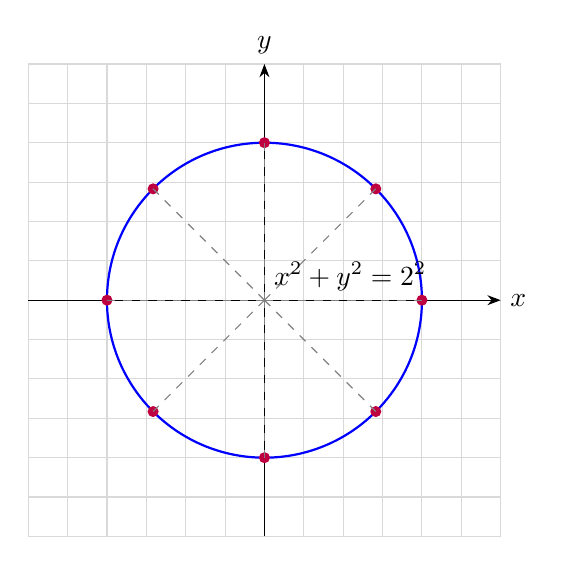
\begin{tikzpicture}[>=Stealth]
\draw[gray!30,step=0.5] (-3,-3) grid (3,3);
\draw[->] (-3,0) -- (3,0) node[right] {$x$};
\draw[->] (0,-3) -- (0,3) node[above] {$y$};
\draw[thick,blue] (0,0) circle (\rad);
\foreach \a in {0,45,...,315} {
  \fill[purple] (\a:\rad) circle (2pt);
  \draw[gray,dashed] (0,0) -- (\a:\rad);
}
\node[above right] at (0,0) {$x^2+y^2=\rad^2$};
\end{tikzpicture}
\end{document}
